% !Mode:: "TeX:UTF-8"
% !TEX program  = xelatex

% \documentclass{cumcmthesis}
\documentclass[withoutpreface,bwprint]{cumcmthesis} %去掉封面与编号页,电子版提交的时候使用。


\usepackage[framemethod=TikZ]{mdframed}
\usepackage{url}   % 网页链接
% \usepackage{subcaption} % 子标题
\title{穿越沙漠路径规划的宽度优先搜索模型}

\begin{document}

    \maketitle
    \begin{abstract}
        本文针对穿越沙漠最优路径规划问题,基于图论、宽度优先搜索、博弈论纳什均衡理论,建立了数学模型,为游戏参与者提供了不同情境下的最优策略。

        我们使用一个五元组\((d,p,f,w,m)\)来描述游戏参与者所处的状态,其中\(d,p,f,w,m\)分别表示游戏参与者所在日期、所处位置、所带食物,所带水和所带资金。游戏开始时游戏参与者处在\((0,1,0,0,10000)\)节点,目标是在\(d\leq\)限定时间内到达\(p=\)终点,同时使\(m\)尽可能的大。状态之间的转移包括前进、停留、挖矿和购买物资四种。

        在第一问中,我们用起点、村庄、矿山和终点构成加权连通图,每条边的权值对应于两个顶点之间的最短路线,我们证明了在已知全部天气时这样的加权图可以代替原地图,减少了节点数,简化了计算。

        在一名玩家且已知全部天气情况时,我们可以具体表示出每一步状态转移对应的水、食物和资金的消耗,利用宽度优先搜索,从只包含\((0,1,0,0,10000)\)的队列开始拓展,
        % 每次从队头取出一个节点,按照状态转移方法拓展出所有可行节点,将他们放入原队列队尾,不断重复直到队列为空。利用宽度优先搜索,我们
        可以找到所有能够从起点在限制时间内到达终点的路径,将他们放入一个以到达终点所保留的资金进行比较的优先队列,就能得到最优策略。

        在第二问中,我们采用估值函数来确定最佳策略,对于游戏中的每一天,已知当天的天气情况,我们都可以计算,对于每一种接下来的选择:停留、购物、挖矿、前进到每一个邻格,分别计算在这种选择下,以后所有天都是晴朗天气和都是高温天气时限制时间内走到终点的最大持有的资金,取一个平均值作为这种选择的预期收益,再以预期收益最大的那种选择作为最优策略。这种计算的方法中,计算终点持有资金时之后的天气情况已经全部设定了,就可以利用第一问的方法去计算,只需要把当前位置当作“不能再以基准价格购物的起点”就行。

        % 在第三问中,我们

\keywords{宽度优先搜索\quad 图搜索\quad 规划模型\quad 纳什均衡}
\end{abstract}

%目录  2019 明确不要目录,我觉得这个规定太好了
%\tableofcontents

%\newpage

\section{问题重述}

穿越沙漠问题是一个在约束条件下求最优解的问题,具体来说,指在给定的地图上,玩家在游戏开始时获得一定的初始资金,可以在起点购买一定数量的水和食物,然后从起点出发,穿过沙漠抵达终点。在穿越沙漠中,玩家所携带的水和食物不能呢超越其最大背负重量,但必须大于等于当天的消耗,从而不至于渴死或者饿死。穿越途中会遇到不同的天气,也可以在矿山获得资金,或者在村庄购买资源,抵达终点之后也可以退回多余的水和食物。游戏要求在规定的时间到达终点,在终点拥有的资金则多多益善。

我们需要建立数学模型解决如下具体问题:

\subsection{问题一}
只有一名玩家,游戏开始时,游戏时间内每天天气情况就全部已知,在此条件下求解一个最优策略,使得到达终点时持有最多的资金。

\subsection{问题二}
只有一名玩家,玩家只知道当天的天气情况,求解一个最优策略,使得玩家能根据当天的天气情况选择当天的行动,使得到达终点时持有最多的资金。

\subsection{问题三}
有$n$名玩家,且多名玩家走相同路线、在同一村庄买物资和在同一矿山挖矿会减少每个人的收益,在玩家知道每天天气和只知道当天天气情况下,分别求解能使达到终点持有最多资金的行动策略。


\section{问题分析}

\subsection{问题一的分析}
问题一中游戏全程的天气情况都是已知的,那么对于每一步的状态转移,我们都能直接计算出这一步状态转移所消耗的资产、水和食物。这样,从起点这一初始状态出发,按照状态转移模型中的条件,我们就可以通过宽度优先搜索,直接搜索出所有起点到终点的完整路径,并找出其中到达终点退还物资后,保留的资产最多的一条路径,这就是我们要求的最优路径。

\subsection{问题二的分析}
相比于问题一,只知道当天的天气情况,我们没法将从当天所在位置开始每种能在时间限制内到达终点的方案,以及到达终点后保留的资金具体的计算出来,但我们可以通过假定天气情况序列来解决这一难题。对于游戏中的每一天,已知当天的天气情况,我们都可以计算,对于每一种接下来的选择:停留、购物、挖矿、前进到每一个邻格,分别计算在这种选择下,以后所有天都是晴朗天气和都是高温天气时限制时间内走到终点的最大持有的资金,取一个平均值作为这种选择的预期收益,再以预期收益最大的那种选择作为最优策略。这种计算的方法中,计算终点持有资金时之后的天气情况已经全部设定了,就可以利用第一问的方法去计算,只需要把当前位置当作“不能再以基准价格购物的起点”就行。

我们注意到,在问题二提供的具体例子第三关和第四关中,都提到了极少出现沙暴天气,从而我们假设不会出现沙暴天气。这样的好处是,在上面的算法中,取所有天都是高温天气得到的收益就是所有可能天气情况下的最小的所有可能路径下的最大可能收益,与之对应,所有天都是晴朗天气得到的收益是所有可能天气情况下的最大的所有可能路径下的最大可能收益。这样,在上面的算法中用这两个收益的平均来评估某路径就是非常合理的。

\subsection{问题三的分析}
相对于前两个问题,问题三的特点在于由单人变成了多人。这时不能简单地走单人时的最优路径,因为当多人走在同一段路或多人在挖矿时,消耗会增大收益会减小。我们注意到在这个游戏面前,$n$个人是完全平等的,即不可能有一个策略能保证某个人一定能严格超过其它人。又注意到,这个游戏追求的是个人利益的最大化,而不是说非要在$n$个人中拿第一名。而且游戏没有禁止玩家之间相互合作。对于玩家们而言,进行充分的合作是有利于保证自己的利益的。所以我们假设玩家之间可以相互交流,并制定出一个对整体最优的策略。进一步,我们觉得在这个游戏中,整体最优的策略很可能就是一个纳什均衡的策略,即哪怕有一个玩家想要偏离整体策略,它的个人收益也不会增加。综上,对于这一问题,我们的方法是用整体最优策略来保证个人利益,具体到某个玩家身上,就是它先要计算出一个整体最优策略,然后和其它玩家沟通,分配大家各自的策略,然后就是按照整体策略中自己的那一部分进行操作就可以了。

第三问还有一个困难的地方,就是在多人的情况下,即使天气全部已知,也不能像第一问一样用关键节点及它们之间的最短路径来简化地图。因为多人的情况下,从一个关键节点到另一个关键节点,走最短路径不一定是消耗最少的。需要尽可能避免和别人走在同一段路上,从而有时需要绕路。不对地图进行简化时,我们依然可以用类似于问题一时的方法通过宽度优先搜索,搜索出所有起点到终点的完整路径,然后得到使n个人的收益之和最大的路径。只是这样做的话,由于没有简化,节点数大大增加,运算量大大增加。我们暂时没有想出比较好的优化的方法。


\section{基本假设}

\begin{enumerate}
    \item 在第二个问题中,不会出现沙暴天气。
    \item 在第三个问题中,玩家之间可以相互沟通相互合作一起制定策略。
\end{enumerate}

\section{变量说明}

\begin{table}[!htbp]
    \caption{符号说明}\label{tab:001} \centering
    \begin{tabular}{ccc}
        \toprule[1.5pt]
        符号 & 意义 & 单位\\
        \midrule[1pt]
        $d$ & 当前日期 & \\
        $p$ & 所在的区域编号 & \\
        $f$ & 所带的食物 & 箱\\
        $w$ & 所带的水 & 箱\\
        $m$ & 所带的资金 & 元\\
        $m_i$ & 第i个人所带的资金 & 元\\
        \(\overrightarrow{D}_i\) & 天气序列排成一系列时间序列 & \\
        \bottomrule[1.5pt]
    \end{tabular}
\end{table}

\section{模型的建立与求解}

我们从图搜索模型的三要素:状态描述、状态转移模型、最终目标来描述这个数学模型。

\subsection{状态的描述}
首先我们讨论状态的描述。我们可以用一个五元组\((d,p,f,w,m)\)来描述当前所处的状态,其中各个符号意义如表\ref{zt},则起始状态可以描述为\((0,1,0,0,10000)\)
\begin{table}[!htbp]
    \caption{五元组中的符号说明}\label{tab:001} \centering
    \begin{tabular}{ccc}
        \toprule[1.5pt]
        符号 & 意义 & 单位\\
        \midrule[1pt]
        $d$ & 当前日期 & \\
        $p$ & 所在的区域编号 & \\
        $f$ & 所带的食物 & 箱\\
        $w$ & 所带的水 & 箱\\
        $m$ & 所带的资金 & 元\\
        $m_i$ & 第i个人所带的资金 & 元\\
        \bottomrule[1.5pt]
    \end{tabular}
    \label{zt}
\end{table}

\subsection{状态的转移模型}
其次我们讨论状态的转移模型。根据题目给出的规则,从每个状态出发,有四种可行的去向:
\begin{enumerate}
    \item 购买物资,这种转移发生在第0天的起点或者第若干天的村庄,\(m\)减小,\(f,w\)相应发生变化。
    \item 前进,从某个地点,前进到相邻的另一个地点,此过程花费1天,并且,消耗掉对应水和食物,\(w,f\)减小。
    \item 停留,在某个地点停留1天。并且,消耗掉对应水和食物,\(w,f\)减小。
    \item 挖矿,在到达矿山的后一天挖矿,此过程花费1天。并且,消耗掉对应水和食物,\(w,f\)减小。
\end{enumerate}

此外,任意一个可行的状态都必须满足\(f\geq 0\)且\(w\geq 0\),不能渴死或者饿死。

沙漠的地图可以抽象为一张无向连通图,我们用邻接矩阵来描述这张图,并以此在程序中判断两地点是否相邻。矩阵\(\mathbf{X}\)展示了该邻接矩阵的局部。

\[
\mathbf{X} = \left(
    \begin{array}{cccccc}
    1 & 1 & 0 & 0 & \ldots & 0\\
    1 & 1 & 1 & 0 & \ldots & 0\\
    0 & 1 & 1 & 1 & \ldots & 0\\
    0 & 0 & 1 & 0 & \ldots & 0\\
    \vdots & \vdots & \vdots & \vdots & \ddots & \vdots\\
    0 & 0 & 0 & 0 & \ldots & 1\\
    \end{array} \right)
\]

\subsection{最终目标}

游戏的最终目标是在\(d\leq\)限定时间内到达\(p=\)终点,同时使\(m\)尽可能的大。在第三问中,涉及到\(n\)个游戏参与者,此时要\(\sum_{i=1}^n m_i\)尽可能的大。

\subsection{对第一问的宽度优先搜索模型}

我们可以很容易地证明,在天气情况全部已知的同一段时间内,从地图的A处到达B处,走最短路径并把多余的时间全部用于在途中停留,这样做所消耗的资源和资金,小于等于走次短路径全程走路所消耗的,所以我们可以忽略次短路径。因此,我们可以先对地图做一些简化。

沙漠的地图可以抽象为一张无向连通图,我们可以通过宽度优先搜索(BFS)来确定起点、村庄、矿山、终点之间的最短路径,就可以把有数十个节点的地图\ref{dt}简化为只有几个顶点的加权连通图\ref{jianhua}。简化过程如图\ref{jianhuaguocheng}所示。

\begin{figure}
    \centering
    \begin{minipage}[c]{0.45\textwidth}
        \centering
        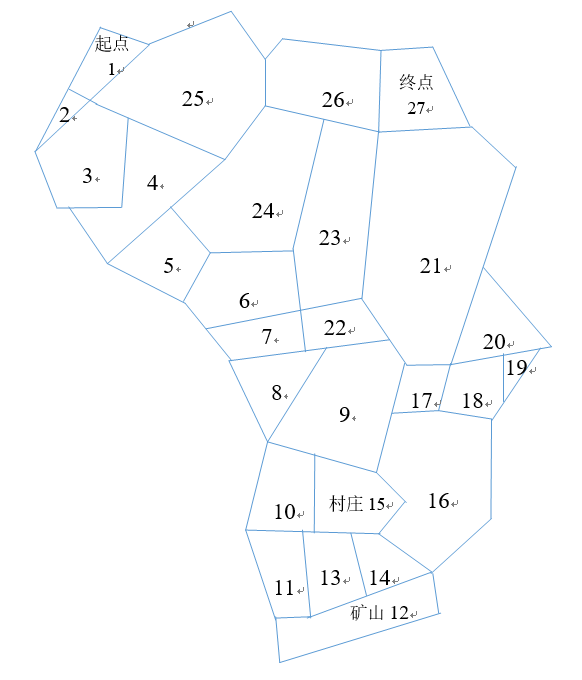
\includegraphics[width=0.95\textwidth]{figures/dt.png}
        \subcaption{第一关地图}
        \label{dt}
    \end{minipage}
    \begin{minipage}[c]{0.45\textwidth}
        \centering
        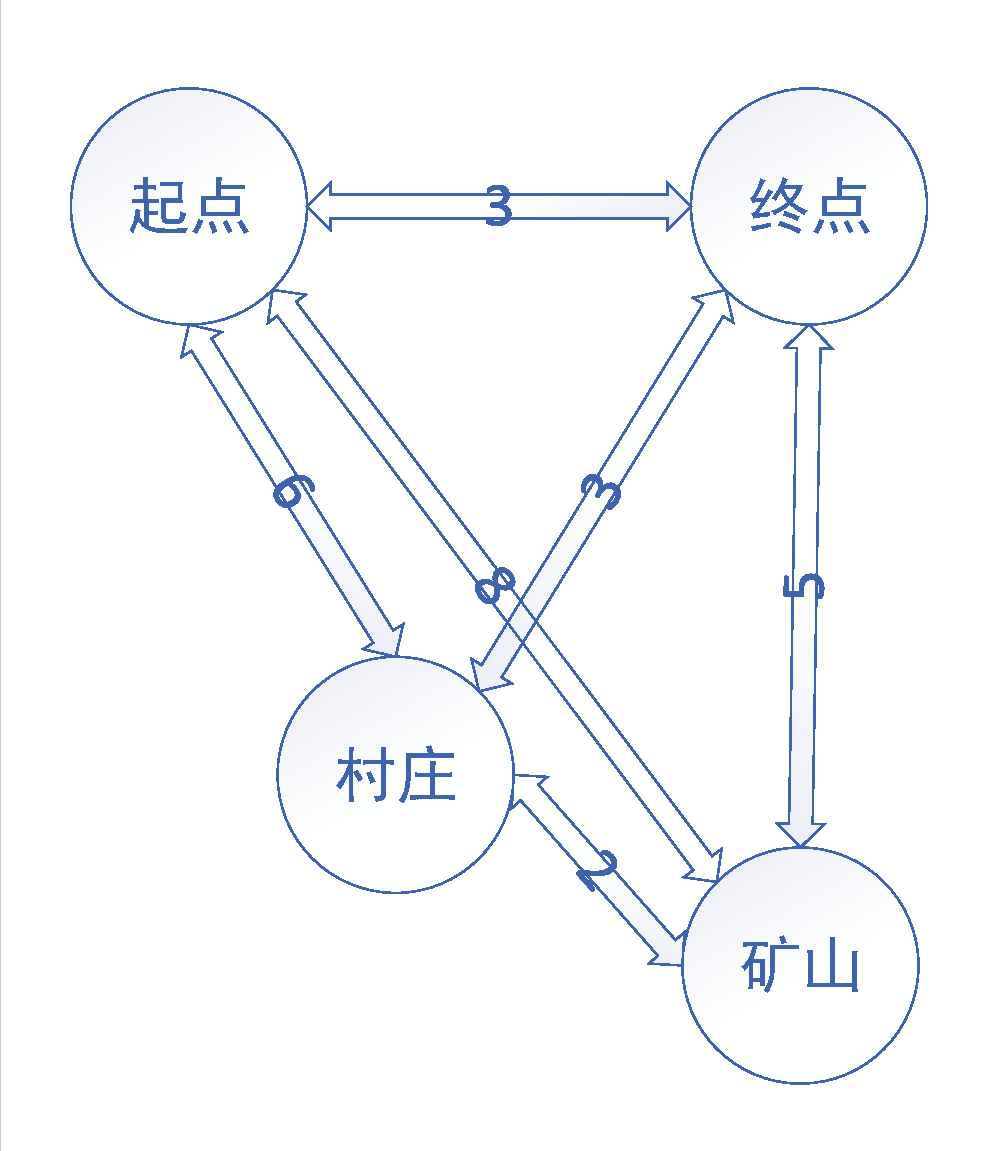
\includegraphics[width=0.95\textwidth]{figures/jianhua.pdf}
        \subcaption{简化后加权图}
        \label{jianhua}
    \end{minipage}
    \caption{用最短路径简化地图}
    \label{jianhuaguocheng}
\end{figure}

对于简化后的地图,状态转移模型也会发生一些变化,优化后的状态转移模型具体如下:

\begin{enumerate}
    \item 购买物资,这种转移发生在第0天的起点或者第若干天的村庄,\(m\)减小,\(f,w\)相应发生变化。
    \item 前进,从某个地点(起点、村庄或者矿山),前进到另一个地点(村庄、矿山或者终点),此过程所花费的时间,\(\geq\)两个地点间最短路径长度,\(\leq\)截止日期--从该地点出发的时间--终点和到达地点的最短路径长度,以保证能在截止日期前到达终点。在时长超过最短路径的前进过程中会有停留,此时优先在这段时间里基础消耗量最大的天气里停留,然后是在基础消耗量次大的天气里停留,最后是基础消耗量最小的天气里停留。并且,消耗掉对应水和食物,\(w,f\)减小。
    \item 停留,在某个地点(起点、村庄或者矿山)停留,此过程所花费的时间,\(\geq\)1天,\(\leq\)截止日期--终点和该地点的最短路径长度,以保证能在截止日期前到达终点。并且,消耗掉对应水和食物,\(w,f\)减小。
    \item 挖矿,在到达矿山的后一天挖矿,此过程所花费的时间,\(\geq\)1天,\(\leq\)截止日期--终点和该矿山的最短路径长度,以保证能在截止日期前到达终点。并且,消耗掉对应水和食物,\(w,f\)减小。
\end{enumerate}

此外,任意一个可行的状态都必须满足\(f\geq 0\)且\(w\geq 0\),不能渴死或者饿死。

\begin{figure}[!htbp]
    \centering
    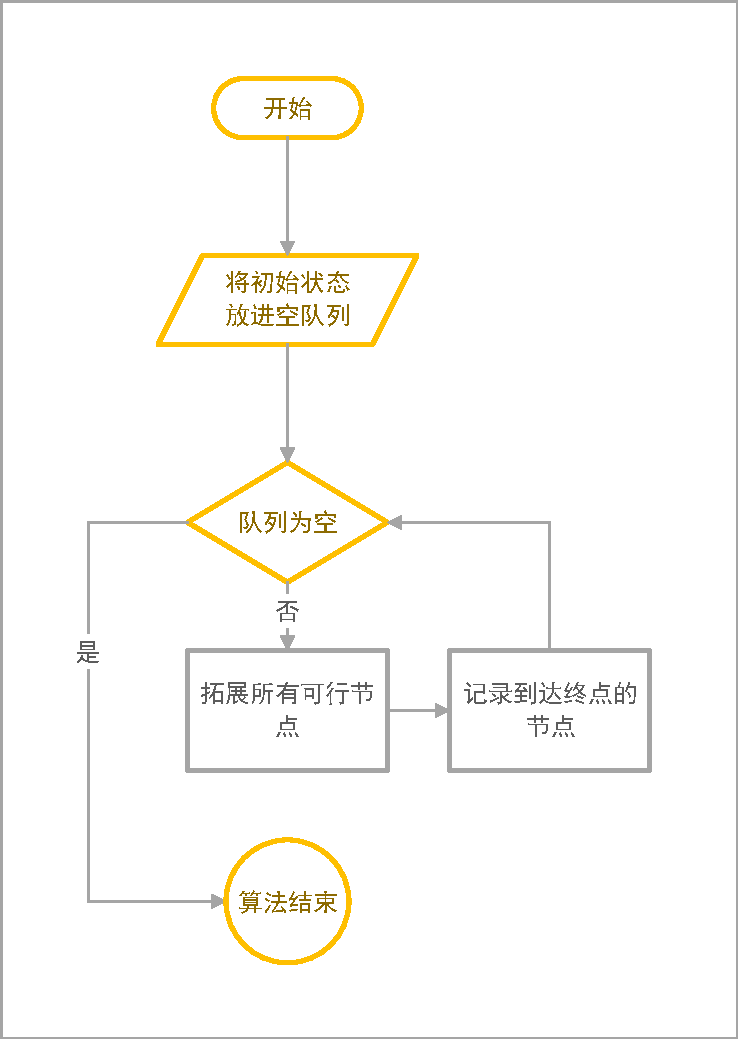
\includegraphics[height=.5\paperheight]{figures/bfs.pdf}
    \caption{宽度优先搜索流程图}
    \label{bfs}
\end{figure}

在只有一名玩家,且已知全部天气情况时,我们可以具体表示出上述每一步状态转移对应的水、食物和资金的消耗。我们对\((d,p,f,w,m)\)中允许的状态组成的状态空间,按以下流程进行宽度优先搜索:
\begin{enumerate}
    \item 构造一个空队列,以及一个优先队列,优先队列以持有的资金\(m\)为排列依据,越多越优先。
    \item 将初始状态\((0,1,0,0,10000)\)节点放进队尾
    \item 从队头取出一个节点,按照上述状态转移规则,进行状态转移,将拓展出所有新的可行节点放入原队列队尾,同时记录状态转移历史
    \item 如果拓展出\(p=\)终点,将它放入优先队列
    \item 不断重复3、4步,直到队列为空,返回优先队列队头元素,算法终止
\end{enumerate}

该返回元素的\(m\)即为最优策略下到终点保留的最多的资产,其状态转移历史即为最优路径。

宽度优先算法可以找到所有能够从起点在限制时间内到达终点的路径,因此能确保所找到的路径是最优的,具有最优性和完备性。为了减小算法复杂度,针对第一关,我们又加入了一些剪枝条件,最终消耗17分钟计算出了第一关的最优解。

剪枝条件如下:
\begin{enumerate}
    \item 枚举在起点购买的水和食物数量时,从到达村庄所需的最小数量开始枚举,并且以达到负重上限为条件(这是因为起点的水和食物价格较便宜)。
    \item 不考虑从起点直接去终点的情况(因为已经找到比直接去终点收益更高的方法)。
    \item 如果a到c的最短路径长度=a到b的最短路径长度+b到c最短路径长度,我们就只考虑a到b的路线,而不考虑从a直接到c的路线,到b了以后再考虑到c或者是其他的路线,这样结果仍是相同的。
    \item 在矿山时,只有当所剩水和食物较少时才考虑去村庄。直接剪掉所剩水和食物或天数不足以到达村庄或终点的情况。
    \item 不考虑除了沙暴以外的在路上停留(因为消耗资源必然变多,而且损失了一天时间)。
    \item 在村庄枚举购买水和食物数量时,以达到负重上限为条件。如果到终点还有剩余的,再加上相应的钱数(可以视作原来在村庄少买了一些)。
\end{enumerate}

\begin{figure}
    \centering
    \begin{minipage}[c]{0.45\textwidth}
        \centering
        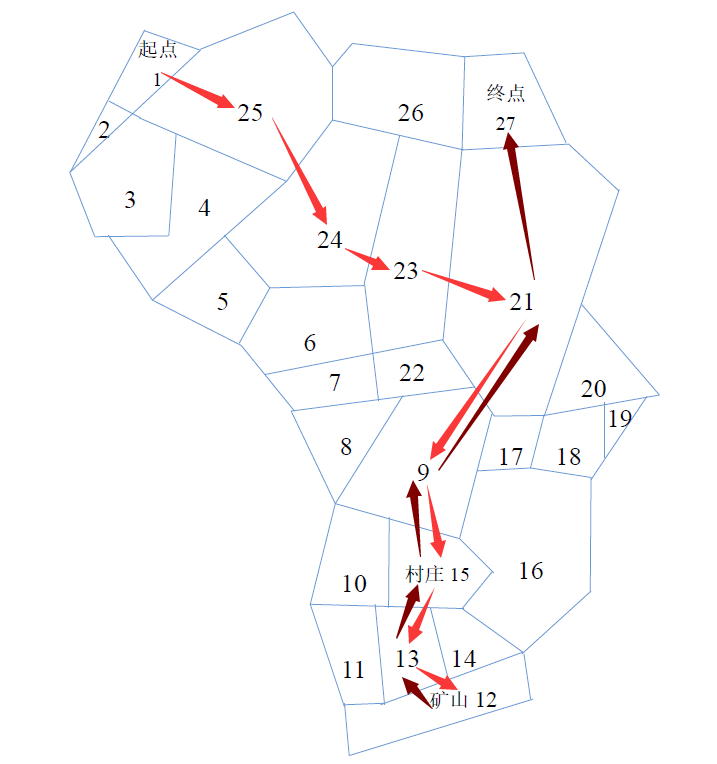
\includegraphics[width=.95\textwidth]{figures/gate1.png}
        \subcaption{第一关最优路径示意图}
        \label{gate1}
    \end{minipage}
    \begin{minipage}[c]{0.45\textwidth}
        \centering
        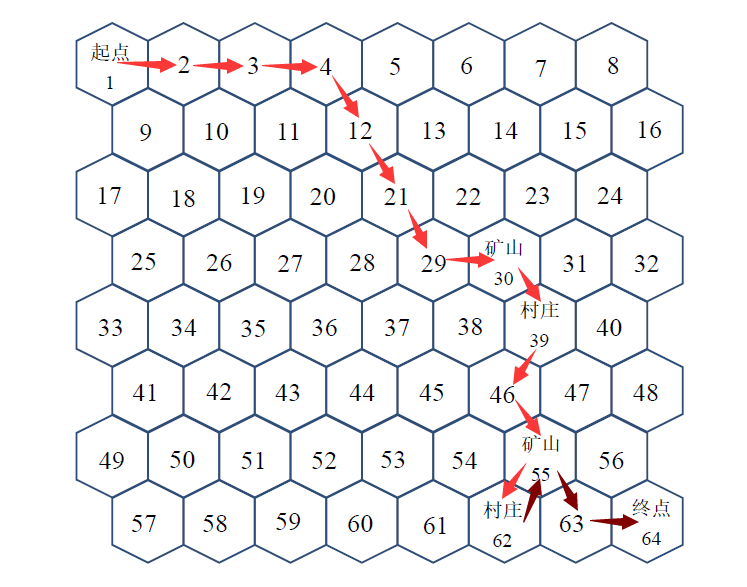
\includegraphics[width=.95\textwidth]{figures/gate2.png}
        \subcaption{第二关最优路径示意图}
        \label{gate2}
    \end{minipage}
    \caption{第一问最优路径示意图}
    \label{q1}
\end{figure}

最后计算出的第一关和第二关的最优路径如图\ref{q1},其到达终点归还水和食物之后的最大保留资金分别是10430元和12700元,同时路径上的计算结果也填到了Result.xlsx中。

\subsection{对第二问的宽度优先搜索估值模型}

相比于问题一,只知道当天的天气情况,我们没法将从当天所在位置开始每种能在时间限制内到达终点的方案,以及到达终点后保留的资金具体的计算出来,但我们已经在第一问中找到了已知天气序列计算最终收益的方法。在第二问里,我们可以通过假定天气情况序列,从而利用第一问方法来解决这一难题。

对于游戏中的每一天,已知当天的天气情况,我们可以对当天以后的天气情况做一些预判。我们把当天以后的天气序列排成一系列时间序列\(\overrightarrow{D}_i\),考虑知道当天天气后,玩家决定前往邻格,或者停留在本地,做出这一行为后,他第二天位于A地

\[
    E m=\sum_i P(\overrightarrow{D}=\overrightarrow{D}_i)m(\overrightarrow{D}_i)
\]

其中\(P(\overrightarrow{D}=\overrightarrow{D}_i)\)表示第i种当天以后的天气序列出现的概率,\(m(\overrightarrow{D}_i)\)表示在天气序列\(\overrightarrow{D}_i\)下,从A地开始,到达终点后所能保留的最大资金数量,\(E m\)就是选择第二天位于A地的话,最后能保留的最大资金的期望。这个期望计算很复杂,但我们可以如下近似。

我们注意到,在问题二提供的具体例子第三关和第四关中,都提到了极少出现沙暴天气,从而我们假设不会出现沙暴天气。这样的好处是,在上面的算法中,取所有天都是高温天气得到的收益就是所有可能天气情况下的最小的所有可能路径下的最大可能收益,与之对应,所有天都是晴朗天气得到的收益是所有可能天气情况下的最大的所有可能路径下的最大可能收益。这些收益可以用第一问的方法计算,只需要把当前位置当作“不能再以基准价格购物的起点”就行

\[
    m(\overrightarrow{D}_{\text{晴朗}}) \leq \sum_i P(\overrightarrow{D}=\overrightarrow{D}_i)m(\overrightarrow{D}_i) \leq m(\overrightarrow{D}_{\text{高温}})
\]

于是,我们可以取今后所有天都是晴朗时的收益、今后所有天都是高温时的收益这两个数的平均值,就能代表做出“明天位于A地”这个选择后的,预期到达终点所持有的资金总量收益。

这提醒我们,可以用这两个收益的平均来评估某路径的好坏,者样我们就有了一个评估函数,返回值就是这个平均值。

我们的策略,就是在知道当天的天气后,分别计算每一种接下来的选择:停留、购物、挖矿、前进到每一个邻格,分别计算在这种选择下的评估函数,选取评估函数最大的那种选择,就是我们在已知当天天气下的最优选择。

以第三关的起点处的选择为例,假设当天天气晴朗,那么,我们可以先计算,如果决定“走到相邻的区域2”,如图\ref{gate3-1}所示,利用上面已有的方法,我们可以分别求出,如果今后天气每天晴朗的最优路线(浅红色箭头),以及到达终点后最大剩余资金9625元,和如果今后天气每天高温的最优路线(深红色箭头),以及到达终点后最大剩余资金9080元,它们的平均值是9352.5,这就是这个决定的预期收益。

\begin{figure}
    \centering
    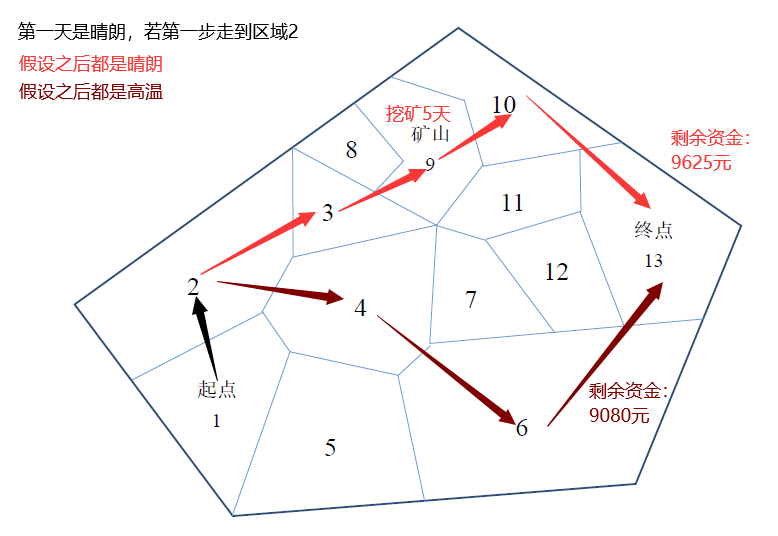
\includegraphics[width=.8\textwidth]{figures/gate3-1.png}
    \caption{前往2号框}
    \label{gate3-1}
\end{figure}

用同样的方法,我们也可求出决定“走到区域4”和“走到区域5”的预期终点最大剩余资金,分别为9510元和9510元,所以,根据策略,我们选择估值函数最大的那种,也就是,当前最优选择是去4或者5,在已知当天(第一天)天气晴朗情况下。

\begin{figure}
    \centering
    \begin{minipage}[c]{0.45\textwidth}
        \centering
        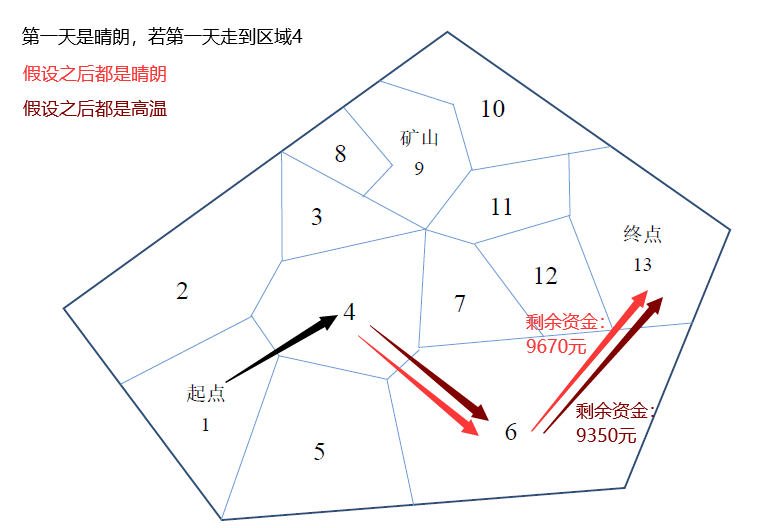
\includegraphics[width=.95\textwidth]{figures/gate3-2.png}
        \subcaption{前往4号框}
        \label{gate3-2}
    \end{minipage}
    \begin{minipage}[c]{0.45\textwidth}
        \centering
        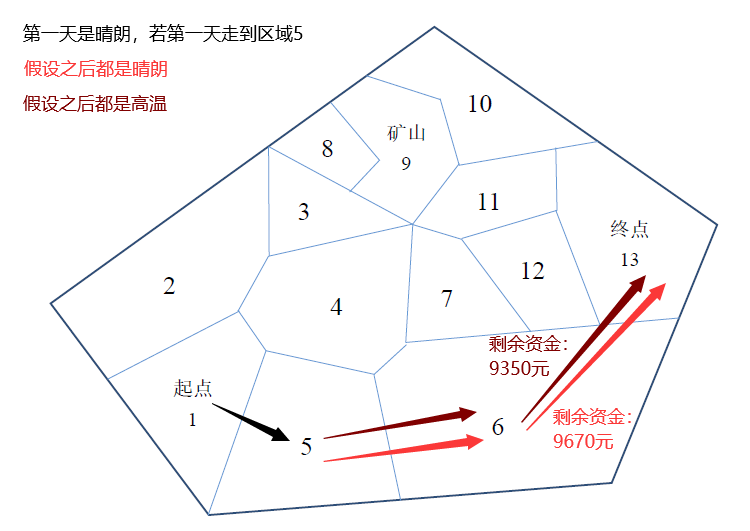
\includegraphics[width=.95\textwidth]{figures/gate3-3.png}
        \subcaption{前往5号框}
        \label{gate3-3}
    \end{minipage}
    \caption{第三关首日已知当天天气晴朗,前往各个邻框的预期收益}
    \label{q2}
\end{figure}

\subsection{问题三的模型}
相对于前两个问题,问题三的特点在于由单人变成了多人。这时不能简单地走单人时的最优路径,因为当多人走在同一段路或多人在挖矿时,消耗会增大收益会减小。我们注意到在这个游戏面前,n个人是完全平等的,即不可能有一个策略能保证某个人一定能严格超过其它人。又注意到,这个游戏追求的是个人利益的最大化,而不是说非要在n个人中拿第一名。而且游戏没有禁止玩家之间相互合作。对于玩家们而言,进行充分的合作是有利于保证自己的利益的。所以我们假设玩家之间可以相互交流,并制定出一个对整体最优的策略。进一步,我们觉得在这个游戏中,整体最优的策略很可能就是一个纳什均衡的策略,即哪怕有一个玩家想要偏离整体策略,它的个人收益也不会增加。综上,对于这一问题,我们的方法是用整体最优策略来保证个人利益,具体到某个玩家身上,就是它先要计算出一个整体最优策略,然后和其它玩家沟通,分配大家各自的策略,然后就是按照整体策略中自己的那一部分进行操作就可以了。

第三问还有一个困难的地方,就是在多人的情况下,即使天气全部已知,也不能像第一问一样用关键节点及它们之间的最短路径来简化地图。因为多人的情况下,从一个关键节点到另一个关键节点,走最短路径不一定是消耗最少的。需要尽可能避免和别人走在同一段路上,从而有时需要绕路。不对地图进行简化时,我们依然可以用类似于问题一时的方法通过宽度优先搜索,搜索出所有起点到终点的完整路径,然后得到使n个人的收益之和最大的路径。只是这样做的话,由于没有简化,节点数大大增加,运算量大大增加。我们暂时没有想出比较好的优化的方法。


% \section{参考文献与引用}

%参考文献
\begin{thebibliography}{9}%宽度9
    % \bibitem[1]{liuhaiyang2013latex}
    % 刘海洋.
    % \newblock \LaTeX {}入门\allowbreak[J].
    % \newblock 电子工业出版社, 北京, 2013.
    \bibitem{mathematical-modeling}
    全国大学生数学建模竞赛论文格式规范 (2020 年 8 月 25 日修改).
    \bibitem{latexstudio} \url{https://www.latexstudio.net}
\end{thebibliography}

\newpage
%附录
\begin{appendices}

\section{第一关宽度优先搜索代码}
\begin{lstlisting}[language=c++]

    #include <iostream>
#include <queue>
#include <vector>
#include <string>
#include <fstream>
using namespace std;
vector<vector<int> > graph;
int weather[31] = {0, 2, 2, 1, 3, 1, 2, 3, 1, 2, 2,
                   3, 2, 1, 2, 2, 2, 3, 3, 2, 2,
                   1, 1, 2, 1, 3, 2, 1, 1, 2, 2};//1-晴朗,2-高温,3-沙暴
int watercost[4] = {0, 5, 8, 10};
int foodcost[4] = {0, 7, 6, 10};

class node
{
public:
    int point;
    string path;
    int step;
    node(int n):point(n){}
};

class state
{
public:
    int p;//当前所在位置
    int d;//日期
    int f;//食物
    int w;//水
    int m;//挖矿次数
    int money;
    int villagebuyfood = 0;//在村庄买的食物
    int villagebuywater = 0;//在村庄买的水
    string path;
    state(int pp, int dd, int ff, int ww, int mm, int moneyy, string pathh) : p(pp), d(dd), f(ff), w(ww), m(mm), money(moneyy), path(pathh){}
    state(){}
};
queue<state> qu;
pair<int, string> bfs(int start, int end)
{
    bool visited[30] = {};
    queue<node> q;
    node s = node(start);
    s.step = 0;
    q.push(s);
    while (!q.empty())
    {
        node t = q.front();
        q.pop();
        visited[t.point] = true;
        if (t.point == end)
        {
            return make_pair(t.step, t.path);
        }
        for (int i = 1; i < graph[t.point].size(); ++i)
        {
            if (visited[graph[t.point][i]])
                continue;
            node nextnode(graph[t.point][i]);
            nextnode.step = t.step + 1;
            nextnode.path = t.path + "-" + to_string(nextnode.point);
            q.push(nextnode);
        }
    }
    return make_pair(-1, "");
}

int main()
{
    for (int i = 0; i <= 27; ++i)
    {
        vector<int> a;
        graph.push_back(a);
    }
    fstream fin("B-1-1邻接表.txt", ios::in);
    for (int i = 1; i <= 27; ++i)
    {
        int a;
        while (fin >> a && a != -1)
        {
            graph[i].push_back(a);
        }
    }
    fin.close();
    pair<int, string> d[6] = {bfs(1, 15), bfs(1, 12), bfs(1, 27), bfs(15, 12), bfs(15, 27), bfs(12, 27)};

    for (int initwater = 98; initwater <= 400; ++initwater)
    {
        for (int initfood = 98; initfood <= 600; ++initfood)
        {
            if (1199 <= (2 * initfood + 3 * initwater) && (2 * initfood + 3 * initwater) <= 1200)
            {
                qu.push(state(1, 0, initfood, initwater, 0, 10000 - 5 * initwater - 10 * initfood, "1"));
            }
            if (2 * initfood + 3 * initwater > 1200)
                break;
        }
    }
    int maxm = 0;
    string anspath;
    state ans;
    while (!qu.empty())
    {
        state t = qu.front();
        qu.pop();
        if (t.d > 30)
            continue;
        if (t.f < 0 || t.w < 0)
        {
            continue;
        }
        //printf("t.d=%d, t.p=%d, t.w=%d, t.f=%d, t.m=%d\n", t.d, t.p, t.w, t.f, t.m);
        switch(t.p)
        {
            case 1:
            {
                //去村庄
                {
                state next = t;
                next.p = 15;
                for (int i = d[0].first; i > 0 && next.d <= 30;)
                {
                    next.d += 1;
                    if (weather[next.d]==3)
                    {
                        next.f -= foodcost[3];
                        next.w -= watercost[3];
                    }
                    else
                    {
                        next.f -= 2 * foodcost[weather[next.d]];
                        next.w -= 2 * watercost[weather[next.d]];
                        i -= 1;
                    }
                }
                next.path = t.path + d[0].second;
                qu.push(next);
                }
                /*
                //去终点
                {
                state next = t;
                next.p = 27;
                for (int i = d[2].first; i > 0;)
                {
                    next.d += 1;
                    if (weather[next.d]==3)
                    {
                        next.f -= foodcost[3];
                        next.w -= watercost[3];
                    }
                    else
                    {
                        next.f -= 2 * foodcost[weather[next.d]];
                        next.w -= 2 * watercost[weather[next.d]];
                        i -= 1;
                    }
                }
                next.path = t.path + d[2].second;
                qu.push(next);
                }
                */

                break;
            }
            case 12:
            {
                if (t.f <= 12 || t.w <= 10 || t.d > 25)
                    break;//无法回到村庄或终点
                if (t.f < 50 || t.w < 50 || t.d == 13)
                {//去村庄,只在食物或水少于50的情况下考虑
                    state next = t;
                    next.p = 15;
                    for (int i = d[3].first; i > 0&&next.d <= 30;)
                    {
                        next.d += 1;
                        if (weather[next.d] == 3)
                        {
                            next.f -= foodcost[3];
                            next.w -= watercost[3];
                        }
                        else
                        {
                            next.f -= 2 * foodcost[weather[next.d]];
                            next.w -= 2 * watercost[weather[next.d]];
                            i -= 1;
                        }
                    }
                    next.path = t.path + "-13-15";
                    qu.push(next);
                }
                //挖一天矿
                {
                    state next = t;
                    next.d += 1;
                    next.m += 1;
                    next.f -= 3 * foodcost[weather[next.d]];
                    next.w -= 3 * watercost[weather[next.d]];
                    next.money += 1000;
                    next.path = t.path + "-mine";
                    qu.push(next);
                }
                if (t.d == 18)
                {//休息一天
                    state next = t;
                    next.d += 1;
                    next.f -= foodcost[weather[next.d]];
                    next.w -= watercost[weather[next.d]];
                    next.path = t.path + "-rest";
                    qu.push(next);
                }
                break;
            }
            case 15:
            {
                if (t.d<=22)
                {//枚举买了多少水和食物,去矿山
                for (int buywater = 0; buywater <= 400; ++buywater)
                {
                    for (int buyfood = 0; buyfood <= 600; ++buyfood)
                    {
                        state next = t;
                        int restmoney = t.money - 10 * buywater - 20 * buyfood;
                        if (2 * (buyfood + t.f) + 3 * (buywater + t.w) >= 1199 &&
                            2 * (buyfood + t.f) + 3 * (buywater + t.w) <= 1200 && restmoney >= 0
                        && (buywater + t.w)>=55 && (buyfood + t.f)>=66)
                        {
                            next.f += buyfood, next.w += buywater, next.money = restmoney;
                            next.villagebuyfood += buyfood, next.villagebuywater += buywater;
                        }
                        else if (2 * (buyfood + t.f) + 3 * (buywater + t.w) > 1200)
                            break;
                        else
                            continue;
                        next.p = 12;
                        for (int i = d[3].first; i > 0&&next.d <= 30;)
                        {
                            next.d += 1;
                            if (weather[next.d] == 3)
                            {
                                next.f -= foodcost[3];
                                next.w -= watercost[3];
                            }
                            else
                            {
                                next.f -= 2 * foodcost[weather[next.d]];
                                next.w -= 2 * watercost[weather[next.d]];
                                i -= 1;
                            }
                        }
                        next.path = t.path + d[3].second;
                        qu.push(next);
                    }
                }
                }

                {//计算好还需要多少水和食物,然后去终点
                    state next = t;
                    next.p = 27;
                    for (int i = d[4].first; i > 0&&next.d <= 30;)
                    {
                        next.d += 1;
                        if (weather[next.d] == 3)
                        {
                            next.f -= foodcost[3];
                            next.w -= watercost[3];
                        }
                        else
                        {
                            next.f -= 2 * foodcost[weather[next.d]];
                            next.w -= 2 * watercost[weather[next.d]];
                            i -= 1;
                        }
                    }
                    if (next.f < 0)
                    {
                        next.money += next.f * 20, next.f = 0;
                    }
                    if (next.w < 0)
                    {
                        next.money += next.w * 10, next.w = 0;
                    }
                    if (next.f > 0)
                    {
                        next.money += 10 * next.f;
                        if (next.f <= next.villagebuyfood)
                            next.money += 10 * next.f;
                        else
                            next.money += 10 * next.villagebuyfood;
                        next.f = 0;
                    }
                    if (next.w > 0)
                    {
                        next.money += 5 * next.w;
                        if (next.w <= next.villagebuywater)
                            next.money += 5 * next.w;
                        else
                            next.money += 5 * next.villagebuywater;
                        next.w = 0;
                    }
                    next.path += d[4].second;
                    qu.push(next);
                }
                break;
            }
            case 27:
            {
                if (maxm < t.money)
                {
                    maxm = t.money;
                    anspath = t.path;
                    ans = t;
                }
                break;
            }
        }
    }
    cout << maxm << " " << anspath << endl;
}
/*
剪枝条件:
1、枚举在起点购买的水和食物数量时,从到达村庄所需的最小数量开始枚举,并且以达到负重上限为条件(这是因为起点的水和食物价格较便宜)。
2、不考虑从起点直接去终点的情况(因为已经找到比直接去终点收益更高的方法)。
3、所有路线在经过村庄的情况下最短距离不变,所以可以认为都从村庄经过,减少了路线的选择。
4、在矿山时,只有当所剩水和食物较少时才考虑去村庄。直接剪掉所剩水和食物或天数不足以到达村庄或终点的情况。
5、不考虑除了沙暴以外的在路上停留(因为消耗资源必然变多,而且损失了一天时间)。
6、在村庄枚举购买水和食物数量时,以达到负重上限为条件。如果到终点还有剩余的,再加上相应的钱数(可以视作原来在村庄少买了一些)。
*/

\end{lstlisting}

\section{第二关宽度优先搜索代码}
\begin{lstlisting}[language=c++]
    #include <iostream>
    #include <queue>
    #include <vector>
    #include <string>
    #include <fstream>
    using namespace std;
    vector<vector<int> > graph;
    int weather[31] = {0, 2, 2, 1, 3, 1, 2, 3, 1, 2, 2,
                       3, 2, 1, 2, 2, 2, 3, 3, 2, 2,
                       1, 1, 2, 1, 3, 2, 1, 1, 2, 2};//1-晴朗,2-高温,3-沙暴
    int watercost[4] = {0, 5, 8, 10};
    int foodcost[4] = {0, 7, 6, 10};
    pair<int, string> d[7][7] = {};
    
    class node
    {
    public:
        int point;
        string path;
        int step;
        node(int n):point(n){}
    };
    
    class state
    {
    public:
        int p;//当前所在位置
        int d;//日期
        int f;//食物
        int w;//水
        int m;//挖矿次数
        int money;
        int villagebuyfood = 0;//在村庄买的食物
        int villagebuywater = 0;//在村庄买的水
        string path;
        state(int pp, int dd, int ff, int ww, int mm, int moneyy, string pathh) : p(pp), d(dd), f(ff), w(ww), m(mm), money(moneyy), path(pathh){}
        state(){}
    };
    queue<state> qu;
    pair<int, string> bfs(int start, int end)
    {
        bool visited[70] = {};
        queue<node> q;
        node s = node(start);
        s.step = 0;
        q.push(s);
        while (!q.empty())
        {
            node t = q.front();
            q.pop();
            visited[t.point] = true;
            if (t.point == end)
            {
                return make_pair(t.step, t.path);
            }
            for (int i = 0; i < graph[t.point].size(); ++i)
            {
                if (visited[graph[t.point][i]])
                    continue;
                node nextnode(graph[t.point][i]);
                nextnode.step = t.step + 1;
                nextnode.path = t.path + "-" + to_string(nextnode.point);
                q.push(nextnode);
            }
        }
        return make_pair(-1, "");
    }
    
    int main()
    {
        for (int i = 0; i <= 64; ++i)
        {
            vector<int> a;
            graph.push_back(a);
        }
        for (int i = 1; i <= 64; ++i)
        {
            if (i % 8 != 1)
            {
                graph[i].push_back(i - 1);
                graph[i - 1].push_back(i);
            }
            if (i > 8)
            {
                if (((i - 1) / 8) % 2 == 1)//偶数行
                {
                    if (i % 16 != 0)
                    {
                        graph[i].push_back(i - 7);
                        graph[i - 7].push_back(i);
                    }
                    graph[i].push_back(i - 8);
                    graph[i - 8].push_back(i);
                }
                if (((i - 1) / 8) % 2 == 0)//奇数行
                {
                    if (i % 16 != 1)
                    {
                        graph[i].push_back(i - 9);
                        graph[i - 9].push_back(i);
                    }
                    graph[i].push_back(i - 8);
                    graph[i - 8].push_back(i);
                }
            }
        }
        d[1][2] = bfs(1, 30), d[1][3] = bfs(1, 39), d[1][4] = bfs(1, 55), d[1][5] = bfs(1, 62), d[1][6] = bfs(1, 64);
        d[2][1] = bfs(30, 1), d[2][3] = bfs(30, 39), d[2][4] = bfs(30, 55), d[2][5] = bfs(30, 62), d[2][6] = bfs(30, 64);
        d[3][1] = bfs(39, 1), d[3][2] = bfs(39, 30), d[3][4] = bfs(39, 55), d[3][5] = bfs(39, 62), d[3][6] = bfs(39, 64);
        d[4][1] = bfs(55, 1), d[4][2] = bfs(55, 30), d[4][3] = bfs(55, 39), d[4][5] = bfs(55, 62), d[4][6] = bfs(55, 64);
        d[5][1] = bfs(62, 1), d[5][2] = bfs(62, 30), d[5][3] = bfs(62, 39), d[5][4] = bfs(62, 55), d[5][6] = bfs(62, 64);
        d[6][1] = bfs(64, 1), d[6][2] = bfs(64, 30), d[6][3] = bfs(64, 39), d[6][4] = bfs(64, 55), d[6][5] = bfs(64, 62);
        
        for (int initwater = 130; initwater <= 400; ++initwater)
        {
            for (int initfood = 122; initfood <= 600; ++initfood)
            {
                if (1199 <= (2 * initfood + 3 * initwater) && (2 * initfood + 3 * initwater) <= 1200)
                {
                    qu.push(state(1, 0, initfood, initwater, 0, 10000 - 5 * initwater - 10 * initfood, "1"));
                }
                if (2 * initfood + 3 * initwater > 1200)
                    break;
            }
        }
        int maxm = 0;
        string anspath;
        state ans;
        while (!qu.empty())
        {
            state t = qu.front();
            qu.pop();
            if (t.d > 30)
                continue;
            if (t.f < 0 || t.w < 0)
            {
                continue;
            }
            //printf("t.d=%d, t.p=%d, t.w=%d, t.f=%d, t.m=%d\n", t.d, t.p, t.w, t.f, t.m);
            switch(t.p)
            {
                case 1:
                {
                    //去矿山30
                    {
                    state next = t;
                    next.p = 30;
                    for (int i = d[1][2].first; i > 0 && next.d <= 30;)
                    {
                        next.d += 1;
                        if (weather[next.d] == 3)
                        {
                            next.f -= foodcost[3];
                            next.w -= watercost[3];
                        }
                        else
                        {
                            next.f -= 2 * foodcost[weather[next.d]];
                            next.w -= 2 * watercost[weather[next.d]];
                            i -= 1;
                        }
                    }
                    next.path = t.path + d[1][2].second;
                    qu.push(next);
                    }
    
                    //去矿山55
                    {
                    state next = t;
                    next.p = 55;
                    for (int i = d[1][4].first; i > 0 && next.d <= 30;)
                    {
                        next.d += 1;
                        if (weather[next.d] == 3)
                        {
                            next.f -= foodcost[3];
                            next.w -= watercost[3];
                        }
                        else
                        {
                            next.f -= 2 * foodcost[weather[next.d]];
                            next.w -= 2 * watercost[weather[next.d]];
                            i -= 1;
                        }
                    }
                    next.path = t.path + d[1][4].second;
                    qu.push(next);
                    }
    
                    //去村庄62
                    {
                    state next = t;
                    next.p = 62;
                    for (int i = d[1][5].first; i > 0 && next.d <= 30;)
                    {
                        next.d += 1;
                        if (weather[next.d] == 3)
                        {
                            next.f -= foodcost[3];
                            next.w -= watercost[3];
                        }
                        else
                        {
                            next.f -= 2 * foodcost[weather[next.d]];
                            next.w -= 2 * watercost[weather[next.d]];
                            i -= 1;
                        }
                    }
                    next.path = t.path + d[1][5].second;
                    qu.push(next);
                    }
                    
                    //去终点64
                    {
                    state next = t;
                    next.p = 64;
                    for (int i = d[1][6].first; i > 0;)
                    {
                        next.d += 1;
                        if (weather[next.d]==3)
                        {
                            next.f -= foodcost[3];
                            next.w -= watercost[3];
                        }
                        else
                        {
                            next.f -= 2 * foodcost[weather[next.d]];
                            next.w -= 2 * watercost[weather[next.d]];
                            i -= 1;
                        }
                    }
                    next.path = t.path + d[1][6].second;
                    qu.push(next);
                    }
                    
    
                    break;
                }
    
                case 30:
                {
                    if (t.f <= 12 || t.w <= 10 || t.d > 26)
                        break;//无法回到村庄或终点
                    if (t.f < 50 || t.w < 50 || t.d == 26)
                    {//去村庄39,只在食物或水少于50的情况下考虑
                        state next = t;
                        next.p = 39;
                        for (int i = d[2][3].first; i > 0&&next.d <= 30;)
                        {
                            next.d += 1;
                            if (weather[next.d] == 3)
                            {
                                next.f -= foodcost[3];
                                next.w -= watercost[3];
                            }
                            else
                            {
                                next.f -= 2 * foodcost[weather[next.d]];
                                next.w -= 2 * watercost[weather[next.d]];
                                i -= 1;
                            }
                        }
                        next.path = t.path + d[2][3].second;
                        qu.push(next);
                    }
                    //挖一天矿
                    {
                        state next = t;
                        next.d += 1;
                        next.m += 1;
                        next.f -= 3 * foodcost[weather[next.d]];
                        next.w -= 3 * watercost[weather[next.d]];
                        next.money += 1000;
                        next.path = t.path + "-mine";
                        qu.push(next);
                    }
                    /*
                    if (t.d == 18)
                    {//休息一天
                        state next = t;
                        next.d += 1;
                        next.f -= foodcost[weather[next.d]];
                        next.w -= watercost[weather[next.d]];
                        next.path = t.path + "-rest";
                        qu.push(next);
                    }
                    */
                    break;
                }
                case 39:
                {
                    if (t.d <= 24)
                    {//枚举买了多少水和食物,去矿山30
                        for (int buywater = 0; buywater <= 400; ++buywater)
                        {
                            for (int buyfood = 0; buyfood <= 600; ++buyfood)
                            {
                                state next = t;
                                int restmoney = t.money - 10 * buywater - 20 * buyfood;
                                if (2 * (buyfood + t.f) + 3 * (buywater + t.w) >= 1199 &&
                                    2 * (buyfood + t.f) + 3 * (buywater + t.w) <= 1200 && restmoney >= 0 && 
                                    (buywater + t.w) >= 41 && (buyfood + t.f) >= 42)
                                {
                                    next.f += buyfood, next.w += buywater, next.money = restmoney;
                                    next.villagebuyfood += buyfood, next.villagebuywater += buywater;
                                }
                                else if (2 * (buyfood + t.f) + 3 * (buywater + t.w) > 1200)
                                    break;
                                else
                                    continue;
                                next.p = 30;
                                for (int i = d[3][2].first; i > 0 && next.d <= 30;)
                                {
                                    next.d += 1;
                                    if (weather[next.d] == 3)
                                    {
                                        next.f -= foodcost[3];
                                        next.w -= watercost[3];
                                    }
                                    else
                                    {
                                        next.f -= 2 * foodcost[weather[next.d]];
                                        next.w -= 2 * watercost[weather[next.d]];
                                        i -= 1;
                                    }
                                }
                                next.path = t.path + d[3][2].second;
                                qu.push(next);
                            }
                        }
                    }
    
                    if (t.d <= 25)
                    {//枚举买了多少水和食物,去矿山55
                        for (int buywater = 0; buywater <= 400; ++buywater)
                        {
                            for (int buyfood = 0; buyfood <= 600; ++buyfood)
                            {
                                state next = t;
                                int restmoney = t.money - 10 * buywater - 20 * buyfood;
                                if (2 * (buyfood + t.f) + 3 * (buywater + t.w) >= 1199 &&
                                    2 * (buyfood + t.f) + 3 * (buywater + t.w) <= 1200 && restmoney >= 0 && 
                                    (buywater + t.w) >= 51 && (buyfood + t.f) >= 54)
                                {
                                    next.f += buyfood, next.w += buywater, next.money = restmoney;
                                    next.villagebuyfood += buyfood, next.villagebuywater += buywater;
                                }
                                else if (2 * (buyfood + t.f) + 3 * (buywater + t.w) > 1200)
                                    break;
                                else
                                    continue;
                                next.p = 55;
                                for (int i = d[3][4].first; i > 0 && next.d <= 30;)
                                {
                                    next.d += 1;
                                    if (weather[next.d] == 3)
                                    {
                                        next.f -= foodcost[3];
                                        next.w -= watercost[3];
                                    }
                                    else
                                    {
                                        next.f -= 2 * foodcost[weather[next.d]];
                                        next.w -= 2 * watercost[weather[next.d]];
                                        i -= 1;
                                    }
                                }
                                next.path = t.path + d[3][4].second;
                                qu.push(next);
                            }
                        }
                    }
    
                    {//计算好还需要多少水和食物,然后去终点
                        state next = t;
                        next.p = 64;
                        for (int i = d[3][6].first; i > 0&&next.d <= 30;)
                        {
                            next.d += 1;
                            if (weather[next.d] == 3)
                            {
                                next.f -= foodcost[3];
                                next.w -= watercost[3];
                            }
                            else
                            {
                                next.f -= 2 * foodcost[weather[next.d]];
                                next.w -= 2 * watercost[weather[next.d]];
                                i -= 1;
                            }
                        }
                        if (next.f < 0)
                        {
                            next.money += next.f * 20, next.f = 0;
                        }
                        if (next.w < 0)
                        {
                            next.money += next.w * 10, next.w = 0;
                        }
                        if (next.f > 0)
                        {
                            next.money += 10 * next.f;
                            if (next.f <= next.villagebuyfood)
                                next.money += 10 * next.f;
                            else
                                next.money += 10 * next.villagebuyfood;
                            next.f = 0;
                        }
                        if (next.w > 0)
                        {
                            next.money += 5 * next.w;
                            if (next.w <= next.villagebuywater)
                                next.money += 5 * next.w;
                            else
                                next.money += 5 * next.villagebuywater;
                            next.w = 0;
                        }
                        next.path += d[3][6].second;
                        qu.push(next);
                    }
                    break;
                }
    
                case 55:
                {
                    if (t.f <= 12 || t.w <= 10 || t.d > 28)
                        break;//无法回到村庄或终点
                    if (t.f < 30 || t.w < 30)
                    {//去村庄62,只在食物或水少于30的情况下考虑
                        state next = t;
                        next.p = 62;
                        for (int i = d[4][5].first; i > 0&&next.d <= 30;)
                        {
                            next.d += 1;
                            if (weather[next.d] == 3)
                            {
                                next.f -= foodcost[3];
                                next.w -= watercost[3];
                            }
                            else
                            {
                                next.f -= 2 * foodcost[weather[next.d]];
                                next.w -= 2 * watercost[weather[next.d]];
                                i -= 1;
                            }
                        }
                        next.path = t.path + d[4][5].second;
                        qu.push(next);
                    }
                    //挖一天矿
                    {
                        state next = t;
                        next.d += 1;
                        next.m += 1;
                        next.f -= 3 * foodcost[weather[next.d]];
                        next.w -= 3 * watercost[weather[next.d]];
                        next.money += 1000;
                        next.path = t.path + "-mine";
                        qu.push(next);
                    }
                    {//计算好还需要多少水和食物,然后去终点
                        state next = t;
                        next.p = 64;
                        for (int i = d[4][6].first; i > 0&&next.d <= 30;)
                        {
                            next.d += 1;
                            if (weather[next.d] == 3)
                            {
                                next.f -= foodcost[3];
                                next.w -= watercost[3];
                            }
                            else
                            {
                                next.f -= 2 * foodcost[weather[next.d]];
                                next.w -= 2 * watercost[weather[next.d]];
                                i -= 1;
                            }
                        }
                        if (next.f < 0 || next.w < 0)
                        {
                            break;
                        }
                        if (next.f > 0)
                        {
                            next.money += 10 * next.f;
                            if (next.f <= next.villagebuyfood)
                                next.money += 10 * next.f;
                            else
                                next.money += 10 * next.villagebuyfood;
                            next.f = 0;
                        }
                        if (next.w > 0)
                        {
                            next.money += 5 * next.w;
                            if (next.w <= next.villagebuywater)
                                next.money += 5 * next.w;
                            else
                                next.money += 5 * next.villagebuywater;
                            next.w = 0;
                        }
                        next.path += d[4][6].second;
                        qu.push(next);
                    }
                    break;
                }
    
                case 62:
                {
                    
                    if (t.d <= 26)
                    {//枚举买了多少水和食物,去矿山55
                        for (int buywater = 0; buywater <= 400; ++buywater)
                        {
                            for (int buyfood = 0; buyfood <= 600; ++buyfood)
                            {
                                state next = t;
                                int restmoney = t.money - 10 * buywater - 20 * buyfood;
                                if (2 * (buyfood + t.f) + 3 * (buywater + t.w) >= 1199 &&
                                    2 * (buyfood + t.f) + 3 * (buywater + t.w) <= 1200 && restmoney >= 0 && 
                                    (buywater + t.w) >= 41 && (buyfood + t.f) >= 42)
                                {
                                    next.f += buyfood, next.w += buywater, next.money = restmoney;
                                    next.villagebuyfood += buyfood, next.villagebuywater += buywater;
                                }
                                else if (2 * (buyfood + t.f) + 3 * (buywater + t.w) > 1200)
                                    break;
                                else
                                    continue;
                                next.p = 55;
                                for (int i = d[5][4].first; i > 0 && next.d <= 30;)
                                {
                                    next.d += 1;
                                    if (weather[next.d] == 3)
                                    {
                                        next.f -= foodcost[3];
                                        next.w -= watercost[3];
                                    }
                                    else
                                    {
                                        next.f -= 2 * foodcost[weather[next.d]];
                                        next.w -= 2 * watercost[weather[next.d]];
                                        i -= 1;
                                    }
                                }
                                next.path = t.path + d[5][4].second;
                                qu.push(next);
                            }
                        }
                    }
    
                    {//计算好还需要多少水和食物,然后去终点
                        state next = t;
                        next.p = 64;
                        for (int i = d[5][6].first; i > 0&&next.d <= 30;)
                        {
                            next.d += 1;
                            if (weather[next.d] == 3)
                            {
                                next.f -= foodcost[3];
                                next.w -= watercost[3];
                            }
                            else
                            {
                                next.f -= 2 * foodcost[weather[next.d]];
                                next.w -= 2 * watercost[weather[next.d]];
                                i -= 1;
                            }
                        }
                        if (next.f < 0)
                        {
                            next.money += next.f * 20, next.f = 0;
                        }
                        if (next.w < 0)
                        {
                            next.money += next.w * 10, next.w = 0;
                        }
                        if (next.f > 0)
                        {
                            next.money += 10 * next.f;
                            if (next.f <= next.villagebuyfood)
                                next.money += 10 * next.f;
                            else
                                next.money += 10 * next.villagebuyfood;
                            next.f = 0;
                        }
                        if (next.w > 0)
                        {
                            next.money += 5 * next.w;
                            if (next.w <= next.villagebuywater)
                                next.money += 5 * next.w;
                            else
                                next.money += 5 * next.villagebuywater;
                            next.w = 0;
                        }
                        next.path += d[5][6].second;
                        qu.push(next);
                    }
                    break;
                }
    
                case 64:
                {
                    if (maxm < t.money)
                    {
                        maxm = t.money;
                        anspath = t.path;
                        ans = t;
                    }
                    break;
                }
            }
        }
        cout << maxm << " " << anspath << endl;
    }
\end{lstlisting}

\section{第三关宽度优先搜索代码}
\begin{lstlisting}[language=c++]
    #include <iostream>
#include <queue>
#include <vector>
#include <string>
#include <fstream>
using namespace std;
vector<vector<int> > graph;
int weather[11] = {};//1-晴朗,2-高温,3-沙暴
int watercost[4] = {0, 3, 9, 10};
int foodcost[4] = {0, 4, 9, 10};

class node
{
public:
    int point;
    string path;
    int step;
    node(int n):point(n){}
};

class state
{
public:
    int p;//当前所在位置
    int d;//日期
    int f;//食物
    int w;//水
    int m;//挖矿次数
    int money;
    int villagebuyfood = 0;//在村庄买的食物
    int villagebuywater = 0;//在村庄买的水
    string path;
    state(int pp, int dd, int ff, int ww, int mm, int moneyy, string pathh) : p(pp), d(dd), f(ff), w(ww), m(mm), money(moneyy), path(pathh){}
    state(){}
};
queue<state> qu;
pair<int, string> bfs(int start, int end)
{
    bool visited[30] = {};
    queue<node> q;
    node s = node(start);
    s.step = 0;
    q.push(s);
    while (!q.empty())
    {
        node t = q.front();
        q.pop();
        visited[t.point] = true;
        if (t.point == end)
        {
            return make_pair(t.step, t.path);
        }
        for (int i = 1; i < graph[t.point].size(); ++i)
        {
            if (visited[graph[t.point][i]])
                continue;
            node nextnode(graph[t.point][i]);
            nextnode.step = t.step + 1;
            nextnode.path = t.path + "-" + to_string(nextnode.point);
            q.push(nextnode);
        }
    }
    return make_pair(-1, "");
}
pair<int, string> d[14][14] = {};

int conutmoney(int start)
{
    for (int initwater = 18; initwater <= 400; ++initwater)
    {
        for (int initfood = 24; initfood <= 600; ++initfood)
        {
            if ((2 * initfood + 3 * initwater) >= 1199 && (2 * initfood + 3 * initwater) <= 1200)
            {
                if (start==1)
                {
                    qu.push(state(start, 1, initfood - foodcost[weather[1]], initwater - watercost[weather[1]],
                                  0, 10000 - 5 * initwater - 10 * initfood, "1-rest"));
                }
                else
                {
                    qu.push(state(start, 1, initfood - 2 * foodcost[weather[1]], initwater - 2 * watercost[weather[1]],
                                  0, 10000 - 5 * initwater - 10 * initfood, "1-" + to_string(start)));
                }
                
            }
            if (2 * initfood + 3 * initwater > 1200)
                break;
        }
    }
    int maxm = 0;
    string anspath;
    state ans;
    while (!qu.empty())
    {
        state t = qu.front();
        qu.pop();
        if (t.d > 10)
            continue;
        if (t.f < 0 || t.w < 0)
        {
            continue;
        }
        //printf("t.d=%d, t.p=%d, t.w=%d, t.f=%d, t.m=%d\n", t.d, t.p, t.w, t.f, t.m);
        if (t.p == start)
            {
                //去矿山
                {
                state next = t;
                next.p = 9;
                for (int i = d[start][9].first; i > 0 && next.d <= 10;)
                {
                    next.d += 1;
                    if (weather[next.d] == 3)
                    {
                        next.f -= foodcost[3];
                        next.w -= watercost[3];
                    }
                    else
                    {
                        next.f -= 2 * foodcost[weather[next.d]];
                        next.w -= 2 * watercost[weather[next.d]];
                        i -= 1;
                    }
                }
                next.path = t.path + d[start][9].second;
                qu.push(next);
                }
                
                //去终点
                {
                state next = t;
                next.p = 13;
                for (int i = d[start][13].first; i > 0 && next.d <= 10;)
                {
                    next.d += 1;
                    if (weather[next.d]==3)
                    {
                        next.f -= foodcost[3];
                        next.w -= watercost[3];
                    }
                    else
                    {
                        next.f -= 2 * foodcost[weather[next.d]];
                        next.w -= 2 * watercost[weather[next.d]];
                        i -= 1;
                    }
                }
                next.path = t.path + d[start][13].second;
                qu.push(next);
                }
            }
        if (t.p == 9)
            {
                if (t.f < 16 || t.w < 12 || t.d > 8)
                    continue;

                if (t.f <= 54 || t.w <= 54 || t.d == 8)
                {//去终点,只在食物或水较少或天数将尽的情况下考虑
                    state next = t;
                    next.p = 13;
                    for (int i = d[9][13].first; i > 0&&next.d <= 10;)
                    {
                        next.d += 1;
                        if (weather[next.d] == 3)
                        {
                            next.f -= foodcost[3];
                            next.w -= watercost[3];
                        }
                        else
                        {
                            next.f -= 2 * foodcost[weather[next.d]];
                            next.w -= 2 * watercost[weather[next.d]];
                            i -= 1;
                        }
                    }
                    next.path = t.path + d[9][13].second;
                    qu.push(next);
                }
                
                //挖一天矿
                {
                    state next = t;
                    next.d += 1;
                    next.m += 1;
                    next.f -= 3 * foodcost[weather[next.d]];
                    next.w -= 3 * watercost[weather[next.d]];
                    next.money += 200;
                    next.path = t.path + "-mine";
                    qu.push(next);
                }
                
                {//休息一天
                    state next = t;
                    next.d += 1;
                    next.f -= foodcost[weather[next.d]];
                    next.w -= watercost[weather[next.d]];
                    next.path = t.path + "-rest";
                    qu.push(next);
                }
            }
            
        if (t.p == 13)
            {
                if (t.f>0)
                {
                    t.money += 10 * t.f;
                }
                if (t.w>0)
                {
                    t.money += 5 * t.w;
                }
                if (maxm < t.money)
                {
                    maxm = t.money;
                    anspath = t.path;
                    ans = t;
                }
            }
        
    }
    cout << maxm << " " << anspath << endl;
    return maxm;
}

int main()
{
    for (int i = 0; i <= 13; ++i)
    {
        vector<int> a;
        graph.push_back(a);
    }
    fstream fin("B-2-3邻接表.txt", ios::in);
    for (int i = 1; i <= 13; ++i)
    {
        int a;
        while (fin >> a && a != -1)
        {
            graph[i].push_back(a);
        }
    }
    fin.close();

    for (int i = 1; i <= 13; ++i)
    {
        for (int j = 1; j <= 13; ++j)
        {
            if (i == j)
                continue;
            d[i][j] = bfs(i, j);
        }
    }

    //第一天是晴天
    weather[1] = 1;
    cout << "第一天是晴天\n";
    //假设之后都是晴天
    for (int i = 2; i <= 10; ++i)
        weather[i] = 1;
    cout << "假设之后都是晴天\n";
    cout << conutmoney(1) << endl;//第一天停留
    cout << conutmoney(2) << endl;//第一天去2号区域
    cout << conutmoney(4) << endl;//第一天去4号区域
    cout << conutmoney(5) << endl;//第一天去5号区域
    //假设之后都是晴天
    for (int i = 2; i <= 10; ++i)
        weather[i] = 2;
    cout << "假设之后都是高温\n";
    cout << conutmoney(1) << endl;//第一天停留
    cout << conutmoney(2) << endl;//第一天去2号区域
    cout << conutmoney(4) << endl;//第一天去4号区域
    cout << conutmoney(5) << endl;//第一天去5号区域
    
    
    //第一天是高温
    weather[1] = 2;
    cout << "第一天是高温\n";
    //假设之后都是晴天
    for (int i = 2; i <= 10; ++i)
        weather[i] = 1;
    cout << "假设之后都是晴天\n";
    cout << conutmoney(1) << endl;//第一天停留
    cout << conutmoney(2) << endl;//第一天去2号区域
    cout << conutmoney(4) << endl;//第一天去4号区域
    cout << conutmoney(5) << endl;//第一天去5号区域
    //假设之后都是晴天
    for (int i = 2; i <= 10; ++i)
        weather[i] = 2;
    cout << "假设之后都是高温\n";
    cout << conutmoney(1) << endl;//第一天停留
    cout << conutmoney(2) << endl;//第一天去2号区域
    cout << conutmoney(4) << endl;//第一天去4号区域
    cout << conutmoney(5) << endl;//第一天去5号区域
}
\end{lstlisting}

\end{appendices}

\end{document} 